%\documentclass[preprint,12pt]{aastex}
\documentclass[preprint2]{aastex}
%\documentclass[iop]{emulateapj}
%\usepackage{subfigure}
\usepackage{natbib}
%not sure I really need these
\usepackage{calrsfs,euscript,mathrsfs,amssymb}
\usepackage{graphicx}
\graphicspath{ {Figures/} }
\usepackage[hyphens]{url}
\usepackage{hyperref}

%not sure what this does
%\usepackage[nomarkers,nolists]{endfloat}

%\usepackage{lineno}
\usepackage[mathlines]{lineno}
\linenumbers

%Jamie added this to have inline colored comments
\newcount\Comments  % 0 suppresses notes to selves in text
\Comments=1   % TODO: set to 0 for final version
\usepackage[usenames,dvipsnames]{xcolor}
\definecolor{darkgreen}{rgb}{0,0.5,0}
\definecolor{purple}{rgb}{1,0,1}
\definecolor{darkpurple}{rgb}{0.5,0,0.5}
\definecolor{lightgreen}{RGB}{135,220,0}

% \kibitz{color}{comment} inserts a colored comment in the text
\newcommand{\kibitz}[2]{\ifnum\Comments=1\textcolor{#1}{#2}\fi}
% add yourself here: 
\newcommand{\jamie}[1]{\kibitz{red}      {[JAM: #1]}}

\newcommand{\myemail}{jcohen@astro.umd.edu}
\newcommand{\HI}{\ion{H}{1}}
\newcommand{\mH}{H$_2$}
\newcommand{\Msun}{$M_\odot$}
\newcommand{\gam}{$\gamma$-ray}
%\newcommand{\lat}{\textit{Fermi}-LAT }
\newcommand{\g}{$\gamma$}
\newcommand{\vdag}{(v)^\dagger}
\newcommand{\kms}{km s$^{-1}$}
\newcommand{\msol}{\hbox{$M_\odot$}}            % Solar mass
\newcommand{\Fermi}{\emph{Fermi }}  % Fermi
\newcommand{\FermiLat}{\emph{Fermi} LAT }     %Fermi LAT
\newcommand{\ptlike}{{\tt pointlike}}
\newcommand{\gtlike}{{\tt gtlike}}
\newcommand{\Gone}{G150.3+4.5}



\shorttitle{G150.3+4.5 GeV paper}
\shortauthors{Cohen, Hays, Hewitt }
\slugcomment{}
% can play with these things to change the margins
%\setlength\topmargin{0in}
%\setlength\headheight{0in}
%\setlength\headsep{0in}
%\setlength\textheight{9in}
%\setlength\textwidth{6.5in}
%\pagestyle{empty}
%\setlength\oddsidemargin{0.5in}
%\setlength\evensidemargin{0.5in}
%\setlength\headheight{77pt}
%\setlength\headsep{0.5in}
\begin{document}
%\begin{doublespace}

\title{Fermi-LAT Observations of Extended Gamma-Ray Emission in the Direction of SNR G150.3+4.5}%Extended Gamma-Ray Emission in the Direction of \Gone~ }
\author{Jamie M. Cohen, Elizabeth Hays, John W. Hewitt}

%maybe don't need this
%\input{authorlist.tex}

\begin{abstract}

We report here a dedicated analysis of the \gam~emission around supernova remnant (SNR) \Gone, observed with the Large Area Telescope (LAT) on board the \textit{Fermi Gamma-Ray Space Telescope}. The Second Catalog of Hard \FermiLat Sources reported detection of a hard spectrum, spatially extended source from 50 GeV - 2TeV, partially overlapping  \Gone. Lowering the energy threshold to 1 GeV we significantly detect a large ($\sigma = 1.40^{\circ} \pm 0.03^{\circ}$) extended \gam~source consistent with the entirety of the radio shell and displaying a power law spectral index of 1.88.  \jamie{all these numbers need to be finalized with the gtlike analysis}
An obtained HI spectrum toward the SNR suggests that the remnant could be one of the closest to us and estimates of its age indicate that \Gone ~may be in the Sedov-Taylor phase \jamie{not sure about this, maybe distance is very uncertain, and hence age as well? My age estimate was $\sim$ 6kyr. Need to think about dynamically young vs. young, fast shocks like which SNR? does dynamically young say something more about the progenitor explosion or surrounding medium?}.  In contrast, the spectrum of the \gam~source is more akin to that of a young, leptonic dominated SNR, although ROSAT X-ray observations show no signs of nonthermal emission coincident typically observed in young SNRs. We discuss alternate origin scenarios for the \gam~emission...
 \jamie{ Should I have the words Pass 8 here somewhere, make it all shorter? move the on board stuff to intro. }

\end{abstract}

%\keywords{catalogs -- gamma rays: general}
\keywords{Supernova Remnants, \g-rays, Cosmic rays, Radio}

%do I need maketitle here? 
%\maketitle
%\clearpage

%%%%%%%%%%%%%%%%%%%%%%%%%%%%%%%%%%%%%%%%%%%%%%%%%%%%%%%%%%%%%%%%
%
%         Introduction 
%
%%%%%%%%%%%%%%%%%%%%%%%%%%%%%%%%%%%%%%%%%%%%%%%%%%%%%%%%%%%%%%%%

\section{Introduction} 


%\citep{2013ApJS..208...17A} testing bib

Something about SNRs, cosmic ray accelerators, radio detections, connection between radio-LAT observations, G150 detection, 2FHL blind detection and SNRs at TeV (all young?), this paper extends the energy down to

We describe the LAT and analysis results in $\S$\ref{sec:LATobs}, detail multiwavelength observations in $\S$\ref{sec:Multiwave}, and discuss various emission origin scenarios in $\S$\ref{sec:Discuss}.
%%%%%%%%%%%%%%%%%%%%%%%%%%%%%%%%%%%%%%%%%%%%%%%%%%%%%%%%%%%%%%%%
%
%         FermiLat  Observations and  Analysis 
%
%%%%%%%%%%%%%%%%%%%%%%%%%%%%%%%%%%%%%%%%%%%%%%%%%%%%%%%%%%%%%%%%
\section{\label{sec:LATobs}\FermiLat  Observations and  Analysis }
\subsection{\label{sec:LATdata}Data Set and Reduction}
\FermiLat is a pair conversion telescope sensitive to high energy \gam s  from 20 MeV to greater than 1 TeV \citep{2FHL}, operating primarily in a sky-survey mode which views  the entire sky every 3 hours. The LAT has wide field of view ($\sim$2.4 sr), a large effective area of $\sim$8200 cm$^2$ above 1 GeV for on axis events and a  68\% containment radius angular resolution  of $\sim$0.8$^\circ$  at 1 GeV. For further details  on the instrument and its performance see \cite{atwood09} and \cite{lat_perf}.

In this analysis, we  analyzed 7 years of Pass 8 data, from August 2nd 2008  to August 2nd 2015. The Pass 8 event reconstruction provides a significantly improved angular resolution \jamie{this is sadly unimportant unless I'm at higher energy or using the PSF types. The P8 total PSF at 1 GeV is about the same as for P7REP. It's the acceptance/effective area that are considerably better at this energy}, acceptance, and background event rejection \citep{atwood13b,atwood13}, all of which lead to an increase in the effective energy range and sensitivity of the LAT. Source class events were analyzed within a 14$^\circ$x14$^\circ$ region centered on SNR \Gone~using the P8R2\_SOURCE\_V6 instrument response functions, with a pixel size of 0.1$^{\circ}$. To reduce contamination from earth limb \gam s, only events with a zenith angle less than 100$^{\circ}$ were included.

For spectral and spatial analysis we utilized both the standard \Fermi Science Tools (version 10-01-01)\footnote[1]{\url{http://fermi.gsfc.nasa.gov/ssc/}} , and the binned maximum likelihood package \ptlike~\citep{Kerr10}. \ptlike~provides methods for simultaneously fitting the spectrum, position, and spatial extension of a source, and  was extensively validated in \cite{Lande12}. Both packages fit a source model, the Galactic diffuse emission, and an isotropic component (which accounts for the background of misclassified charged particles and the extragalactic diffuse \gam background)\footnote[2]{\url{http://fermi.gsfc.nasa.gov/ssc/data/access/lat/BackgroundModels.html}} to the observations.  In this analysis, we used the standard Galactic diffuse ring-hybrid model, scaled  for Pass 8 analysis, gll{\_}iem{\_}v06.fits, and for the isotropic emission,  we used iso{\_}P8R2{\_}SOURCE{\_}V6{\_}v06.txt, extrapolated to 2 TeV as in \cite{2FHL}.

In our source model for the region, we included sources from the third \FermiLat catalog \citep[3FGL]{3FGL} within 15$^\circ$ of the center of our region of interest (RoI). We replaced the position and spectrum of any 3FGL pulsars in the region with their corresponding counterpart  from the LAT 2nd pulsar catalog \citep{2PC}.  Residual emission unaccounted for by 3FGL sources is present in the RoI due to the increased time range and different energy selection with respect to that in 3FGL. We added to the RoI several point sources to account for this unmodeled emission and minimize the global residuals.\jamie{do I need to say more about these sources? should I mention adding them automatially and iteraively based on TS maps and reference SNRcat/2FHL? How close is the closest source? Mention this and use as an argument for not saying much more about them}.  The normalization and spectral index of sources within 5$^{\circ}$ of the center of the RoI were free to vary, whereas all other source parameters were fixed. A preliminary likelihood fit of the RoI was performed, and  sources with a test statistic (TS) $<$ 9 (TS is defined as,  ${\rm TS}=2~{\rm Log}(\mathcal{L}_1 / \mathcal{L}_0)$ where $\mathcal{L}_1$ 
 is the likelihood of source plus background and  $\mathcal{L}_0$ that of just the background) were removed from the model. 

\subsection{\label{sec:LATmorph}Morphological Analysis}
Studying the spatial extension of sources with the LAT is non-trivial due to the energy-dependent point spread function (PSF) and strong diffuse emission present in the Galactic plane. To strike a balance between the best angular resolution and minimal diffuse contamination, we restrict our morphological analysis to energies between 1 GeV and  1 TeV. We divide this energy range into 12\jamie{4bpd} logarithmically spaced bins for both \ptlike~and \gtlike~binned likelihood analyses. 

Three  3FGL sources are located within the extent of \Gone. 3FGL J0425.8+5600, located approximately 0.6$^\circ$ from the center of the SNR, is the closest of the three sources and is described with a power law spectrum of index $\Gamma = 2.35\pm 0.17$  in the 3FGL catalog. The closest radio source to 3FGL J0425.8+5600 is NVSS J042719+560823, at 0.25° away (Ref?). 3FGL J0423.5+5442, exhibits a power law spectral index, $\Gamma = 2.63\pm 0.15$, with no clear multiwavelength source association. Finally, 3FGL J0426.7+5437 has a pulsar-like spectrum, yet it is located about 0.8$^{\circ}$ from the center of the SNR. In a timing survey performed with the 100-m  Effelsberg radio telescope, \cite{Barr13} were unable to detect pulsations from the source down to a limiting flux density of $\sim$ 0.1 mJy. We discuss this source and potential emission scenarios further in $\S$\ref{sec:Dist}). 

In our analysis, we removed 3FGL J0425.8+5600 and 3FGL J0423.5+544 from the RoI, but kept 3FGL J0426.7+5437 in the model since preliminary analyses showed clear positive residual emission at the position of the source if it was removed from the RoI. Figure \ref{fig:1GeV_resTSmap} shows a residual TS map for the region around \Gone. This point source detection-significance map was created by placing a point source modeled with a power law with photon index, $\Gamma$ = 2 at each pixel and gives the significance of detecting a point source at each location above the background. \jamie{add something somwhere about contamination with J0426 being another reason for restricting the energy range?}

%put file name in {} to get it to compile with dots in the name!
%for png, have to use pdfchain
\begin{figure}[!ht]
	\begin{centering}
		\includegraphics[width=\columnwidth]{{G150_1GeV_resTsmap_radio_noLabs}.pdf}
		\caption{Background subtracted residual TS map with 0.1$^\circ$x0.1$^\circ$ pixels for fixed index $\Gamma$ = 2 above 1 GeV, centered on SNR \Gone. The orange circle and shading show the fit radius and 1$\sigma$ errors for the extended source, the orange cross  shows the position of 3FGL J0426.7+5437 (included in the background model) and blue circle is the extent of the radio SNR. 
			\label{fig:1GeV_resTSmap}}
	\end{centering}
\end{figure}

\begin{figure}[!ht]
	\begin{centering}
		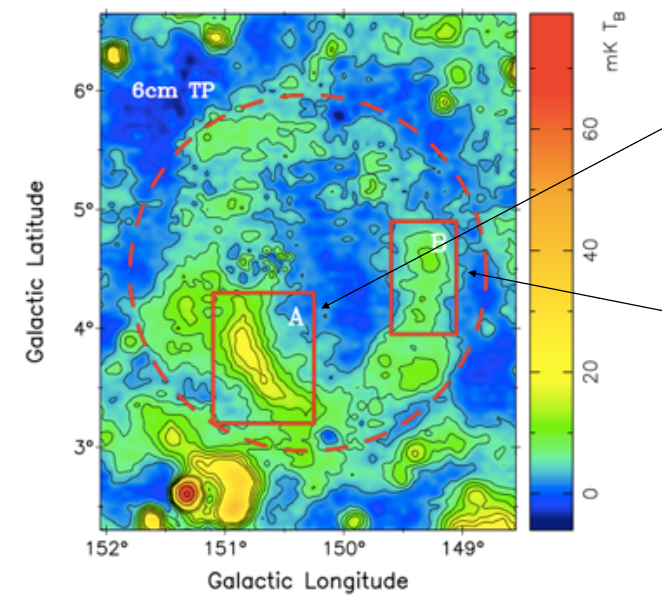
\includegraphics[width=\columnwidth]{Figures/G150_GaoHan.png}
		\caption{This is just a filler image for now while testing things out \citep{Gao14}
			\label{fig:GaoRad}}
	\end{centering}
\end{figure}

We modeled the excess emission in the direction of \Gone with a uniform intensity radially-symmetric disk, simultaneously fitting the spatial and spectral components of the model model via \ptlike. We initialized the  extension with a seed radius, $\sigma$ = 0.1$^\circ$ and initial position centered on the radio position of \Gone. The significance of extension  \jamie{don't need a table for just disk hypothesis right? but maybe need to say something about the disk being a better model than 3 (or more) point sources (I think) I tried adding more sources on top of the 3FGL sources and there's no significant residual). where to say something about testing searching for point sources overlapping the extended source and trying to fit an extended source on top as well? in this table give the disk model with best spectral spatial params, TS, TSext  dof, LL, then the model with just the 3 3FGL sources (no disk) spectrum of each, TS, dof + LL ( didn't relocalize the se sources)}

Fill in more about the TS of these sources at 1 GeV prior to removing them and adding in G150 as well as how they're insiginif when added on top of the extended source. Tried fitting and additional extended source that looks like the 2FHL ans this was insignif (I think this negates the need to try splitting the remnant). Different spatial models also not signif at 1 GeV. refit extension of G150 after adding in nearby sources. No templates since the radio we have is too weak.


\subsection{\label{sec:LATspec}Spectral Analysis}
Describe gtlike  results, spectral models tested (broken PL? no need to since it looks so power law esque?). No break observed, hard spectra increasing to TeV

how many energy bins
\subsection{\label{sec:LATsys}Systematics}
Bracketing IRFs and diffuse systematics study still need to be done


%%%%%%%%%%%%%%%%%%%%%%%%%%%%%%%%%%%%%%%%%%%%%%%%%%%%%%%%%%%%%%%%
%
%         Multiwavelength  Observations and  Analysis 
%
%%%%%%%%%%%%%%%%%%%%%%%%%%%%%%%%%%%%%%%%%%%%%%%%%%%%%%%%%%%%%%%%

\section{\label{sec:Multiwave}Multiwavelength  Observations and  Analysis }
Not sure yet if I'll need separate sections
\subsection{\label{sec:Radio}Radio}
I don't think we're presenting any new Radio analysis, just rehashing previous results, showing radio maps overlaid on GeV, so maybe this is really discussion.
\citep{Gao14}
\subsection{\label{sec:HI}HI}
\subsection{\label{sec:CO}CO}
Make CO overlay maps for the possible velocities. Only issue is that Dame 2001 only goes up to 5 deg. Other CO data that covers better to use? Planck?
\subsection{\label{sec:Xray}X-ray}
No diffuse nonthermal X-ray emission observed by ROSAT. No point sources near the center? Should a pulsar be near the center? How to quantify this? Can we place a limit on something like density with an upper limit on X-ray emission? What about other x-ray telescopes?

%%%%%%%%%%%%%%%%%%%%%%%%%%%%%%%%%%%%%%%%%%%%%%%%%%%%%%%%%%%%%%%%
%
%         Discussion and Results
%
%%%%%%%%%%%%%%%%%%%%%%%%%%%%%%%%%%%%%%%%%%%%%%%%%%%%%%%%%%%%%%%%
\section{\label{sec:Discuss}Discussion and Results}
\subsection{\label{sec:What}What is it?}
Size + HI suggest that near distance corresponding to different HI velocities suggest it's aged, spectrum looks more like young SNR (hard + no GeV break ). Is it a weird young remnant or weird aged one? Leptonic dominated if young, hadronic dominated if older? Something about nearby dense clouds masking hadronic emission? Maybe this is only true for MeV cosmic rays that are screened out though and it would only mask the pion bump, but not this higher energy emission?

PWN or SNR. Can we rule out PWN? See W41 paper, MSH 11-61A, Fabios recent G326 work (no, he just tries to use the PSF types and testing different model templates to try to disentangle SNR from PWN)?

No PSR candidate near center (should it be near the center? Depends on age)
Is there some limit we can place on the PWN based on not seeing the pulsar? Like on Edot? OR something like Mattana et al. 2009 correlation between  $\mathrm{flux_x / flux_g \propto}$   Edot? 

Assume it's in Sedov phase based on size + near distance, and calculate age, upper limit on Edot base on lack of x-ray flux? Or maybe if I assume the sources is the PWN and GeV radius is PWN radius, then can I estimate Edot based on size and evolution inside  SNR?

If we assume close distance, age is only $\approx$ 5kyr, maybe this is a transitional SNR? What do others like this look like? Puppis A? Gamma Cygni is a similar age too.something 


\subsection{\label{sec:Dist}Distance Considerations}
probably doesn't need to be a different section. 
\subsection{\label{secModel}Nonthermal Modeling}
I think I could get a working model with naima running pretty quickly, is it worth it?
%%%%%%%%%%%%%%%%%%%%%%%%%%%%%%%%%%%%%%%%%%%%%%%%%%%%%%%%%%%%%%%%
%
%         Conclusion
%
%%%%%%%%%%%%%%%%%%%%%%%%%%%%%%%%%%%%%%%%%%%%%%%%%%%%%%%%%%%%%%%%
\section{\label{sec:Conc}Conclusions}



%%%%%%%%%%%%%%%%%%%%%%%%%%%%%%%%%%%%%%%%%%%%%%%%%%%%%%%%%%`%%%%%%
%
%         bib
%
%%%%%%%%%%%%%%%%%%%%%%%%%%%%%%%%%%%%%%%%%%%%%%%%%%%%%%%%%%%%%%%%
\bibliographystyle{apj}
\bibliography{biblio.bib}
%\bibliography{test.bib}

%\end{doublespace}

\end{document}